\documentclass[10pt]{article}
\usepackage[a4paper,margin=1.9cm]{geometry}
\usepackage{amsmath,amssymb}
\usepackage{graphicx}
\graphicspath{{../}{./}}
\usepackage{float}
\usepackage[dvipsnames]{xcolor}
\usepackage{enumitem}
\usepackage{titlesec}
\usepackage[hidelinks]{hyperref}

% --- compact layout ---
\setlist[itemize]{leftmargin=1.35em,itemsep=1pt,topsep=2pt,parsep=0pt}
\setlength{\parindent}{0pt}
\setlength{\parskip}{3pt}
\titlespacing*{\section}{0pt}{6pt}{3pt}
\titlespacing*{\subsection}{0pt}{4pt}{2pt}
\titleformat{\section}{\normalfont\large\bfseries\color{RoyalBlue}}{\thesection.}{0.5em}{}
\titleformat{\subsection}{\normalfont\bfseries}{}{0em}{}

\newcommand{\code}[1]{\texttt{\small #1}}
\newcommand{\file}[1]{\textcolor{RoyalBlue}{\texttt{\small #1}}}

% \docheader{title}{subtitle}
\newcommand{\docheader}[2]{%
  \begin{center}
    {\LARGE\bfseries #1}\\[2pt]
    {\small #2}
  \end{center}
  \vspace{-4pt}\hrule\vspace{6pt}
}

\begin{document}

\docheader{Adora PINN --- Step 5: Mock inversion testset}%
{As-built notes \quad$\cdot$\quad Ivan Milic \quad$\cdot$\quad 2026-09-20 \quad$\cdot$\quad step 5 of pinn/plan.md}

The mock inversion testset --- the Stokes observations the PINN will invert --- is a crop of a prepared
synthetic cube, \file{/dat/milic/adora\_synth/test.npz.npy} $(1536{\times}1536{\times}4{\times}201)$: the
first $384{\times}384$ pixels, every 3rd, giving \textbf{$128{\times}128$ pixels at 48\,km horizontal
spacing} (the original 16\,km $\times3$; it will matter for 3D hydrostatic equilibrium later). It is a
magnetized MURaM field ($V$ up to $\pm16$, granular continuum), synthesized with the same Adora RT as the
forward model, so its Stokes units and wavelength grid (Fe I 6301/6302, 201 vac points) match the PINN's
directly. \textbf{Saved to \file{/dat/milic/adora\_pinn\_develop/inversion\_testset.npz}} (keys \code{I\_obs},
\code{waves}, \code{dx\_km}=\code{dy\_km}=48). Against it, the initial model (the pretrained FAL-C field,
non-magnetic) has misfit RMS$(\text{model}-\text{obs})/\langle I_c\rangle$ of $I\,0.20$, $Q\,1.2{\times}10^{-3}$,
$U\,1.2{\times}10^{-3}$, $V\,9.3{\times}10^{-3}$ --- $V$ entirely missing since the model has $B{=}0$ --- which
is the signal the step-6 losses will drive down. Builder \file{pinn/make\_inversion\_testset.py}; notebook
\file{pinn/step5\_testset.ipynb}.

\begin{figure}[h]
\centering
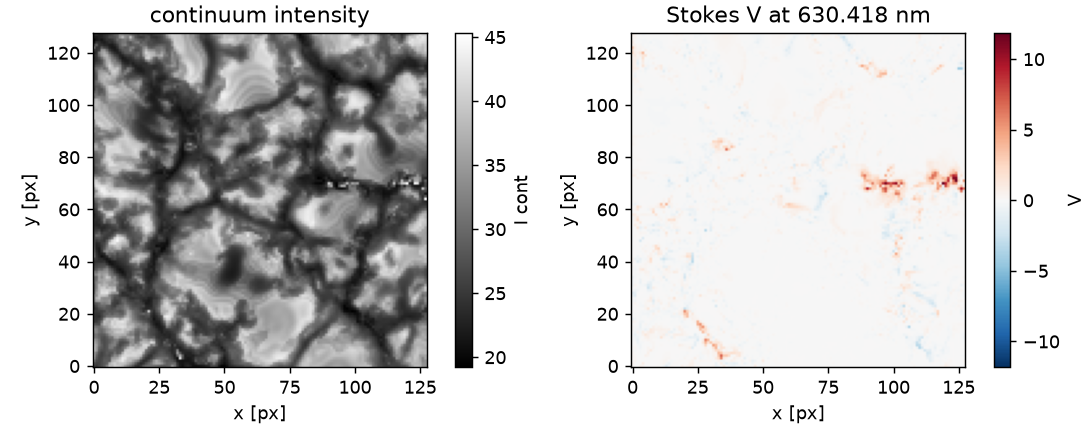
\includegraphics[width=0.86\linewidth]{fig_step5_obs.png}\\[1pt]
{\small\itshape Observations: continuum granulation (left) and the Stokes $V$ polarity map (right).}
\end{figure}

\begin{figure}[h]
\centering
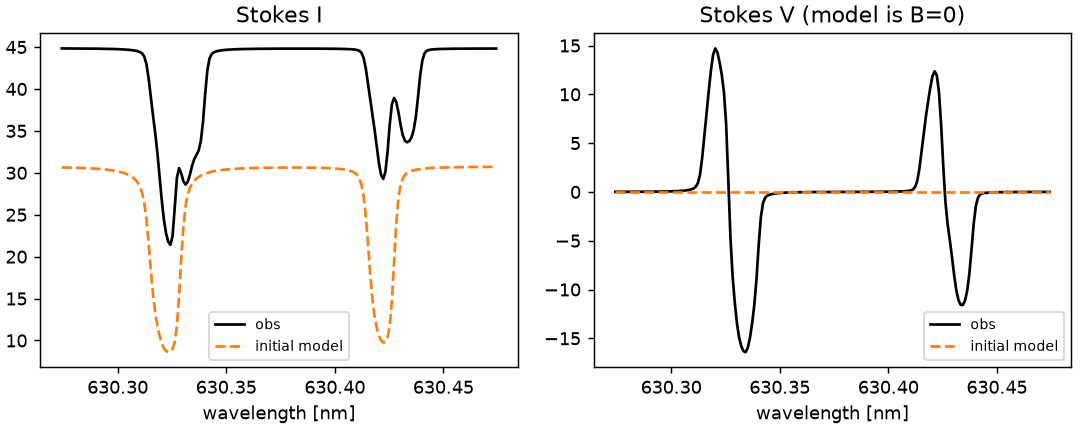
\includegraphics[width=0.86\linewidth]{fig_step5_misfit.png}\\[1pt]
{\small\itshape Initial model vs.\ observations at the most strongly polarised pixel: Stokes $I$ differs and
Stokes $V$ is absent in the non-magnetic starting model --- the starting point of the inversion.}
\end{figure}

\end{document}
